\documentclass{article}
\usepackage[utf8]{inputenc}
\usepackage{fancyhdr}
\usepackage{lastpage}
\usepackage{amsfonts}
\usepackage{amsmath}
\usepackage{amssymb}
\usepackage{bm}
\usepackage{tikz}
\usepackage{tikz-qtree}

\usetikzlibrary{shapes,positioning}
\usepackage{graphicx}
\usepackage{float}
\usepackage[shortlabels]{enumitem}
\usepackage[noabbrev, capitalise]{cleveref}
\usepackage{geometry}
 \geometry{
 a4paper,
 top=20mm,
 bottom=25mm,
 left=25mm,
 right=25mm,
 }

% define your IDs here:
\newcommand{\firststudentid}{307871228}
\newcommand{\secondstudentid}{204617963}

\pagestyle{fancy}
\fancyhf{}
\rhead{Written Solution for Assignment 2}
\chead{\firststudentid \qquad \secondstudentid}
\lhead{Natural Language Processing}
\rfoot{Page \thepage \hspace{1pt} of \pageref{LastPage}}
\renewcommand{\footrulewidth}{1pt}

\setlength{\parindent}{0pt}
\setlength{\parskip}{1em}
\renewcommand{\baselinestretch}{1.25}

\renewcommand{\thesubsection}{\thesection.\alph{subsection}}
\renewcommand{\thesubsubsection}{\thesubsection.\roman{subsubsection}}

\begin{document}
%%%%%%%%%%%%%%%%%%%%% 1 %%%%%%%%%%%%%%%%%%%%%%%
\section{Word-Level Neural Bi-gram Language Model}
\subsection{} %%%%%%%%1a
\begin{equation*}
    J = CE(y, \hat{y}) = -\sum_{i} y_{i}log(\hat{y}_{i}) = -log(\frac{e^{\theta_{i}}}{\sum_{j}e^{\theta_{j}}}) = log(\sum_{j}e^{\theta_{j}}) - \theta_{i}
\end{equation*}
\begin{equation*}
\hat{y} = softmax(\theta)
\end{equation*}
\begin{equation*}
\hat{y_{i}} = softmax(\theta_{i}) = \frac{e^{\theta_{i}}}{\sum_{j}e^{\theta_{j}}}
\end{equation*}
$\nabla_{\theta_{i}} J = \frac{\partial J}{\partial \theta_{i}} = \frac{e^{\theta_{i}}}{\sum_{j}e^{\theta_{j}}} -1 =\hat{y}_{i} -1 $

$\nabla_{\theta_{j \neq i}} J = \frac{\partial J}{\partial \theta_{j \neq i}} = \frac{e^{\theta_{j}}}{\sum_{j}e^{\theta_{j}}} = \hat{y_{j}}$
\begin{equation*}
\implies \nabla_{\theta} J = \frac{\partial J}{\partial \theta} = \hat{y} - y
\end{equation*}

\subsection{} %%%%%%%%%1b
\begin{equation*}
J = CE(y, \hat{y}) = -\sum_{i}{y_{i}log(\hat{y}_{i})}
\end{equation*}
\begin{equation*}
h = \sigma(xW_{1}+b_{1})
\end{equation*}
\begin{equation*}
\hat{y} = \text{softmax}(hW_{2}+b_{2})
\end{equation*}
denote
\begin{equation*}
p = hW_{2}+b_{2}
\end{equation*}
\begin{equation*}
q = xW_{1}+b_{1}
\end{equation*}
then
\begin{equation*}
\frac{\partial J }{\partial x}  = \frac{\partial J }{\partial p} \cdot \frac{\partial p}{\partial h} \cdot \frac{\partial h}{\partial q} \cdot \frac{\partial q}{\partial x}
\end{equation*}
\begin{enumerate}
\item
    $\frac{\partial J }{\partial p} = \hat{y} - y$
\item
    $\frac{\partial p}{\partial h} = \frac{\partial (hW_{2}+b_{2})}{\partial h} = W_{2}$
\item
    $\frac{\partial h}{\partial q} = \frac{\partial \sigma(q)}{\partial q} = \frac{\partial \frac{1}{1+exp(-q)}}{\partial q} = \frac{exp(-q)}{(1+exp(-q))^{2}} = \frac{1}{1+exp(-q)} \cdot \frac{exp(-q)}{1+exp(-q)} = h \cdot (1-h)$
\item
    $\frac{\partial q}{\partial x} = \frac{\partial (xW_{1}+b_{1})}{\partial x} = W_{1}$
\end{enumerate}
\begin{equation*}
    \implies  \frac{\partial J }{\partial x} = (\hat{y} - y) \cdot W_{2} \cdot h \cdot (1-h) \cdot W_{1}
\end{equation*}

\subsection{} %%%%%%%%%1c
(code)

\subsection{} %%%%%%%%%1d
(code)\\\\
\textbf{dev perplexity :} 112.81714028757537


%%%%%%%%%%%%%%%%%%%%% 2 %%%%%%%%%%%%%%%%%%%%%%%
\section{Theoretical Inquiry of a Simple RNN Language Model}
\subsection{} %%%%%%%%%2a
\begin{equation*}
    e^{(t)}=x^{(t)}L
\end{equation*}
\begin{equation*}
    h^{(t)}=\sigma(h^{(t-1)}H + e^{(t)}I + b_{1})
\end{equation*}
\begin{equation*}
    \hat{y}^{(t)}=\text{softmax}(h^{(t)}U+b_{2})
\end{equation*}
\begin{equation*}
    J^{(t)}(\theta)=CE(y^{(t)}, \hat{y}^{(t)}) = - \sum_{i=1}^{|V|}(y_{i}^{(t)}\cdot log(\hat{y_{i}}^{(t)}))
\end{equation*}
\begin{itemize}
    \item $\frac{\partial J^{(t)} }{\partial U} =
     \frac{\partial J^{(t)} }{\partial \hat{y}^{(t)}} \cdot \frac{\partial \hat{y}^{(t)}}{\partial U} = (\hat{y}^{(t)} - y^{(t)}) \cdot h^{(t)}$
    \item $\frac{\partial J^{(t)} }{\partial L_{x^{(t)}}} =
    \frac{\partial J^{(t)} }{\partial \hat{y}^{(t)}} \cdot
    \frac{\partial \hat{y}^{(t)}}{\partial h^{(t)}} \cdot
    \frac{\partial h^{(t)}}{\partial e^{(t)}} \cdot
    \frac{\partial e^{(t)}}{\partial L_{x^{(t)}}} =
    (\hat{y}^{(t)} - y^{(t)}) \cdot U \cdot h^{(t)} \cdot (1 - h^{(t)})$
    \item $\frac{\partial J^{(t)} }{\partial I}\vert_{(t)}  =
    \frac{\partial J^{(t)} }{\partial \hat{y}^{(t)}} \cdot \frac{\partial \hat{y}^{(t)}}{\partial h^{(t)}} \cdot \frac{\partial h^{(t)}}{\partial e^{(t)}} \cdot \frac{\partial e^{(t)}}{\partial I}\vert_{(t)} =
    (\hat{y}^{(t)} - y^{(t)}) \cdot U \cdot h^{(t)} \cdot (1 - h^{(t)}) \cdot x^{(t)}L$
    \item  $\frac{\partial J^{(t)} }{\partial H}\vert_{(t)} = \frac{\partial J^{(t)} }{\partial \hat{y}^{(t)}} \cdot \frac{\partial \hat{y}^{(t)}}{\partial h^{(t)}} \cdot \frac{\partial h^{(t)}}{\partial e^{(t)}} \cdot \frac{\partial e^{(t)}}{\partial H}\vert_{(t)} =
    (\hat{y}^{(t)} - y^{(t)}) \cdot U \cdot h^{(t)} \cdot (1 - h^{(t)}) \cdot h^{(t-1)}$
    \item $\delta^{(t-1)} = \frac{\partial J^{(t)} }{\partial h^{(t-1)}} = \frac{\partial J^{(t)} }{\partial \hat{y}^{(t)}} \cdot \frac{\partial \hat{y}^{(t)}}{\partial h^{(t)}} \cdot \frac{\partial h^{(t)}}{\partial h^{(t-1)}} = (\hat{y}^{(t)} - y^{(t)}) \cdot U \cdot h^{(t)} \cdot (1 - h^{(t)}) \cdot H$
\end{itemize}

\subsection{} %%%%%%%%%2b
\subsubsection{Unrolled network for 3 time-steps}
\tikzset{ell/.style={circle,draw,inner sep=0pt,text width=1cm,align=center}}
\begin{tikzpicture}
    \node[ell] (h3) at (0,0) {$h^{(t-3)}$};
    \node[ell] (h2) at (2,0) {$h^{(t-2)}$};
    \node[ell] (h1) at (4,0) {$h^{(t-1)}$};
    \node[ell] (h) at (6,0) {$h^{(t)}$};
    \node[ell] (x2) at (2,-2) {$x^{(t-2)}$};
    \node[ell] (x1) at (4,-2) {$x^{(t-1)}$};
    \node[ell] (x) at (6,-2) {$x^{(t)}$};
    \node[ell] (y2) at (2,2) {$\hat{y}^{(t-2)}$};
    \node[ell] (y1) at (4,2) {$\hat{y}^{(t-1)}$};
    \node[ell] (y) at (6,2) {$\hat{y}^{(t)}$};
    \node[ell] (dpts) at (8,0) {$\dots$};
    \draw[->] (x2) -- (h2);
    \draw[->] (x1) -- (h1);
    \draw[->] (x) -- (h);
    \draw[->] (h2) -- (h1);
    \draw[->] (h1) -- (h);
    \draw[->] (h3) -- (h2);
    \draw[->] (h) -- (y);
    \draw[->] (h1) -- (y1);
    \draw[->] (h2) -- (y2);
    \draw[->] (h) -- (dpts);
\end{tikzpicture}


\subsubsection{"back-propagation-through-time" gradients}
\begin{itemize}
    \item $\frac{\partial J^{(t)} }{\partial L_{x^{(t-1)}}} =  \frac{\partial J^{(t)} }{\partial \hat{y}^{(t)}} \cdot \frac{\partial \hat{y}^{(t)}}{\partial h^{(t)}} \cdot \frac{\partial h^{(t)}}{\partial e^{(t)}} \cdot \frac{\partial e^{(t)}}{\partial L_{x^{(t-1)}}} =
    (\hat{y}^{(t)} - y^{(t)}) \cdot U \cdot h^{(t)} \cdot (1 - h^{(t)}) \cdot W \cdot h^{(t-1)}$
    \item $\frac{\partial J^{(t)} }{\partial H} \vert_{(t-1)} =  \frac{\partial J^{(t)} }{\partial \hat{y}^{(t)}} \cdot \frac{\partial \hat{y}^{(t)}}{\partial h^{(t)}} \cdot \frac{\partial h^{(t)}}{\partial e^{(t)}} \cdot \frac{\partial e^{(t)}}{\partial H} \vert_{(t-1)} =
    (\hat{y}^{(t)} - y^{(t)}) \cdot U \cdot h^{(t)} \cdot (1 - h^{(t)}) \cdot W \cdot h^{(t-2)}$
    \item $\frac{\partial J^{(t)} }{\partial I} \vert_{(t-1)} =  \frac{\partial J^{(t)} }{\partial \hat{y}^{(t)}} \cdot \frac{\partial \hat{y}^{(t)}}{\partial h^{(t)}} \cdot \frac{\partial h^{(t)}}{\partial e^{(t)}} \cdot \frac{\partial e^{(t)}}{\partial I} \vert_{(t-1)} =
    (\hat{y}^{(t)} - y^{(t)}) \cdot U \cdot h^{(t)} \cdot (1 - h^{(t)}) \cdot W \cdot h^{(t-3)}$
    \item $\frac{\partial J^{(t)} }{\partial b_{1}} \vert_{(t-1)} =  \frac{\partial J^{(t)} }{\partial \hat{y}^{(t)}} \cdot \frac{\partial \hat{y}^{(t)}}{\partial h^{(t)}} \cdot \frac{\partial h^{(t)}}{\partial e^{(t)}} \cdot \frac{\partial e^{(t)}}{\partial b_{1}} \vert_{(t-1)} =
    (\hat{y}^{(t)} - y^{(t)}) \cdot U \cdot h^{(t)} \cdot (1 - h^{(t)})$

\end{itemize}
%%%%%%%%%%%%%%%%%%%%%%%% 3 %%%%%%%%%%%%%%%%%%%%%%%%
\section{Generating Shakespeare Using a Character-level Language Model} %3
\subsection{}
\textbf{Character-based language model advantage:}
\begin{itemize}
    \item It can generate or recognize words that are not present in the training vocabulary by composing them from known characters. This makes them more robust when dealing with rare or specialized terms that may not be present in the training data of a word-based model.
    \item Better identifing and correcting misspaelled and typos.
\end{itemize}
\textbf{Word-based language model advantage:}
\begin{itemize}
    \item Not 'making up' words.
    \item Better context and semantic Understanding: Word-based models capture the meaning of a text at a higher level of abstraction. MOre coherent and contextually appropriate responses.
    \item Computational Efficiency: Word-based models are computationally more efficient than character-based models, as they deal with larger units of text.
\end{itemize}
\subsection{Training-loss plot}
\begin{figure}[h]
\centering
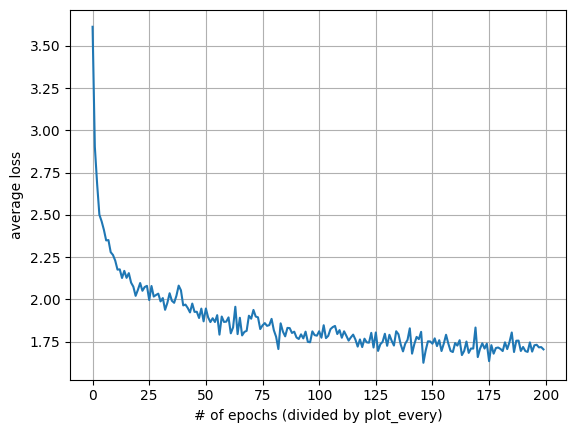
\includegraphics[width=0.6\textwidth]{ims/q3.png}
\caption{Training-loss}
\end{figure}
  %%%%%%%%%%%%%%%%%%%%%%%% 4 %%%%%%%%%%%%%%%%%%%%%%%%
\section{Perplexity}
% \setcounter{subsection}{4}
\subsection{} %%%%%%%4a
we will show:
\begin{equation*}
    2^{\frac{1}{M}\sum_{i=1}^{M}log_2P(s_{i}|s_{1}...s_{i-1})} = e^{\frac{1}{M}\sum_{i=1}^{M}lnP(s_{i}|s_{1}...s_{i-1})}
\end{equation*}

proof:

$2^{\frac{1}{M}\sum_{i=1}^{M}log_2P(s_{i}|s_{1}...s_{i-1})} = 2^{\frac{1}{M}log_2P(s_{1}|s_{1})}  2^{\frac{1}{M}log_2P(s_{2}|s_{1}s_{2})} ... 2^{\frac{1}{M}log_2P(s_{M}|s_{1}...s_{M})} = $

$ = P(s_{1}|s_{1})^{\frac{1}{M}} P(s_{2}|s_{1}s_{2})^{\frac{1}{M}} ... P(s_{M}|s_{1}...s_{M})^{\frac{1}{M}} = $

$ = e^{\frac{1}{M}lnP(s_{1}|s_{1})} e^{\frac{1}{M}lnP(s_{2}|s_{1}s_{2})}  ...  e^{\frac{1}{M}lnP(s_{M}|s_{1}...s_{M})} = e^{\frac{1}{M}\sum_{i=1}^{M}lnP(s_{i}|s_{1}...s_{i-1})}$
\subsection{} %%%%%%%%%4b
\textbf{bi-gram model}
\begin{itemize}
\item \textbf{Shakespeare perplexity:} 7.504480691937161
\item \textbf{Wikipedia perplexity:} 30.17933100905446
\end{itemize}
\textbf{Char-based bi-gram model}
\begin{itemize}
\item \textbf{Shakespeare perplexity:} 6.769117782221575
\item \textbf{Wikipedia perplexity:} 16.2687740098086
\end{itemize}
\subsection{} %%%%%%%%%4c
The first model is a word-based bi-gram model, and the second model is a char-based bi-gram model.
Though we were expecting the char-based model to be better on Shakespeare passege
and the word-based model to be better on Wikipedia passege (in terms of perplexity),
we were surprised to see that both models did better on Shakespeare passege.
The char-based model is more robust to rare words and was trained on Shakespeare corpus, so
the results are not surprising. On the other hand, the word-based model wasn't trained on Shakespeare corpus,
so we were expecting it to do better on Wikipedia passege.
We can think about few reasons for that:

\begin{itemize}
    \item Consistency of Language: "Shakespeare's language" is more consistent
    and constrained compared to the diversed range of topics and writing styles
    found in a single passage from Wikipedia. So based on the context and words in a peragraph,
    both models might predict better on Shakespeare's "strang" words.
    \item The Wikipedia
\end{itemize}

%%%%%%%%%%%%%%%%%%%%%%%% 5 %%%%%%%%%%%%%%%%%%%%%%%%
\section{Deep Averaging Networks}
\subsection{} %%%%%%%5a
\quad (5.a)
\begin{figure}[h]
\centering
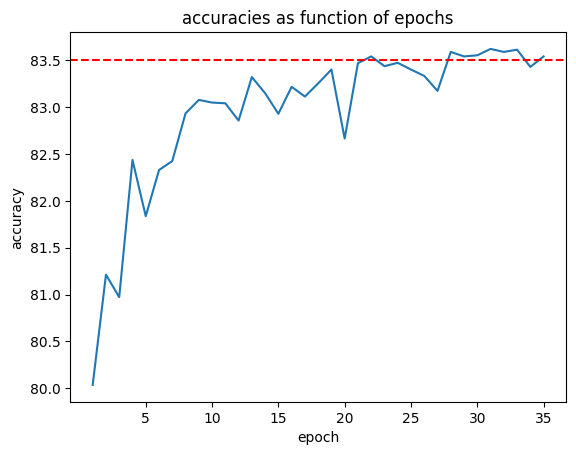
\includegraphics[width=0.6\textwidth]{ims/5a.png}
\caption{Accuracy as a function of number of epochs}
\end{figure}
\subsection{} %%%%%%%5b
\quad (5.b)
\begin{figure}[h]
\centering
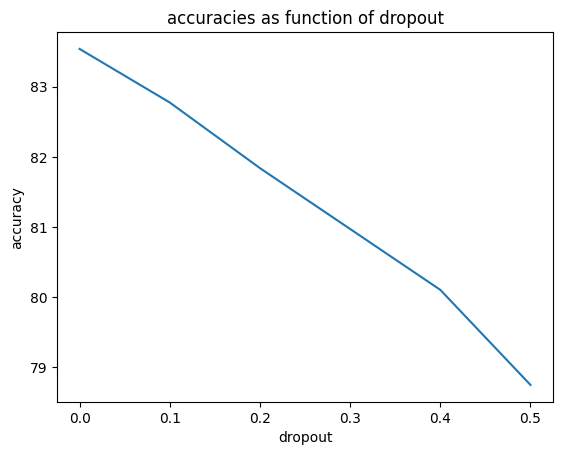
\includegraphics[width=0.6\textwidth]{ims/5b.png}
\caption{Accuracy as a function of dropout rate}
\end{figure}
\subsection{} %%%%%%%5c
\quad (5.c)
\begin{figure}[h]
\centering
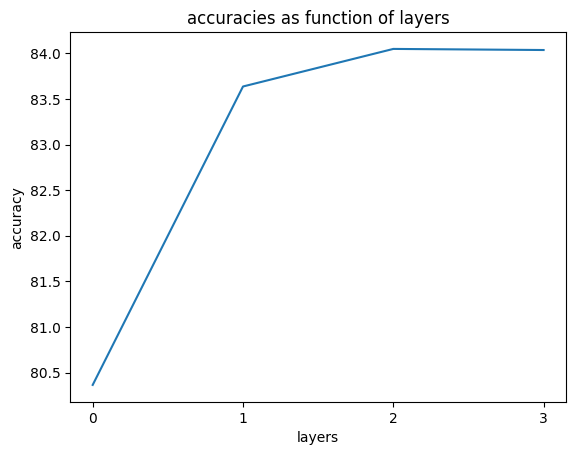
\includegraphics[width=0.6\textwidth]{ims/5c.png}
\caption{Accuracy as a function of number of hidden layers}
\end{figure}
\subsection{} %%%%%%%5d
\quad (5.d)
\begin{figure}[h]
\centering
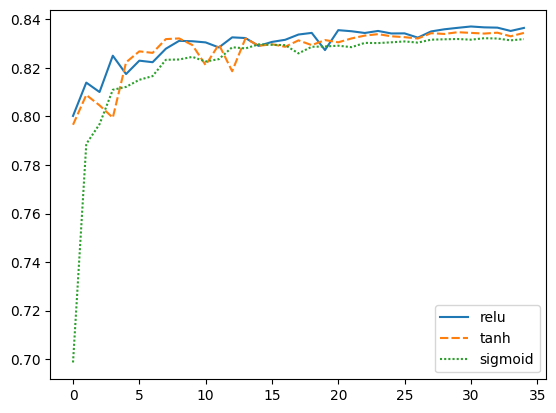
\includegraphics[width=0.6\textwidth]{ims/5d.png}
\caption{Accuracy across epoch}
\end{figure}
\subsection{} %%%%%%%5e
\begin{enumerate}
    \item "This is the latest entry in the long series of films with the French agent,
    O.S.S. 117 (the French answer to James Bond). The series was launched in the early 1950's,
    and spawned at least eight films (none of which was ever released in the U.S.).
    'O.S.S.117:Cairo,Nest Of Spies' is a breezy little comedy that should not...repeat NOT,
    be taken too seriously.
    Our protagonist finds himself in the middle of a spy chase in Egypt (with Morroco
    doing stand in for Egypt) to find out about a long lost friend. What follows is the
    standard James Bond/Inspector Cloussou kind of antics. Although our man is something of
    an overt xenophobe,sexist,homophobe, it's treated as pure farce (as I said,
    don't take it too seriously). Although there is a bit of rough language \& cartoon violence,
    it's basically okay for older kids (ages 12 \& up). As previously stated in the subject
    line, just sit back,pass the popcorn \& just enjoy."\\\\
    \textbf{Predicted:} 0 (negative)\\
    \textbf{Actual:} 1 (positive)\\
    \textbf{Explanation:} the words "should not...repeat NOT", "pure farce", "xenophobe,sexist,homophobe", "rough language \& cartoon violence" and "don't take it too seriously" are negative words.\\
    \item "This is a really sad, and touching movie! It deals with the subject of child abuse.
    It\'s really sad, but mostly a true story, because it happens everyday.
    Elijah Wood and Joseph Mazzello play the two children or Lorraine Bracco, a single mother who just tries to
    make a home for them. While living with her parents, a man, who likes to be called "The King"
    comes into their life. He hits the youngest boy, Bobby, but the two brothers vow not to tell
    their mother. But finally she finds out, after the Bobby is hurt badly. The end kind of ruined
    it for me, because it is so totally unbelievable. But, except for that, I love the movie."\\\\
    \textbf{Predicted:} 0 (negative)\\
    \textbf{Actual: 1} (positive)\\
    \textbf{Explanation:} the words "really sad", "hurt badly", "ruined" and "unbelievable" are negative words.\\
    \item "These days, writers, directors and producers are relying more and more on the "surprise" ending.
    The old art of bringing a movie to closure, taking all of the information we have learned through out the
    movie and bringing it to a nice complete ending, has been lost. Now what we have is a movie that,
    no matter how complex, detailed, or frivolous, can be wrapped up in 5 minutes. It was all in his/her head.
    That explanation is the director\'s safety net. If all else fails, or if the writing wasn\'t that good,
    or if we ran out of money to complete the movie, we can always say "it was all in his/her head" and end
    the movie that way. The audience will buy it because, well, none of us are psychologists, and none of
    us are suffering from schizophrenia (not that we know about) so we take the story and believe it.
    After all, the mind is a powerful thing. Some movies have pulled it off. But those movies are the
    reason why we are getting more and more of these crap endings. Every director/writer now thinks
    they can pull it off because, well, Fight Club did it and it made a lot of money. So we get movies like
    The Machinist, Secret Window, Identity, and this movie (just to name a few)."
    \\\\
    \textbf{Predicted:} 1 (positive)\\
    \textbf{Actual:} 0 (negative)\\
    \textbf{Explanation:} the words ""surprise" ending", "nice complete ending", "The audience will buy it", "pull it off" are positive words.
    \item "It could be easy to complain about the quality of this movie (you don't have to throw cartloads of
    money at a movie to make it good, nor will it guarantee that it is worth watching) but I think that is
    totally missing the point. If your expecting fast cars, T\&A or a movie that will spell itself out
    for you then don't watch this, you'll be disappointed and dumbfounded.<br /><br />This movie was thoroughly
    enjoyable, kept us on the edge of our seats and made us really think. The writer obviously put a lot of
    thought and research behind this movie and it shows through the end, just remember to keep an open mind.
    <br /><br />Note: the school scenes were all filmed at McMaster University and most of the rest was done
    in Toronto."\\\\
    \textbf{Predicted:} 0 (negative)\\
    \textbf{Actual:} 1 (positive)\\
    \textbf{Explanation:} the words "totally missing the point", "disappointed and dumbfounded" are negative words. The begining of the review use negative words, but the end of the review use positive words.\\

    \item "Intended as light entertainment, this film is indeed successful as such during its first half,
    but then succumbs to a rapidly foundering script that drops it down. Harry (Judd Nelson), a "reformed"
    burglar, and Daphne (Gina Gershon), an aspiring actress, are employed as live window mannequins at a
    department store where one evening they are late in leaving and are locked within, whereupon they witness,
    from their less than protective glass observation point, an apparent homicide occurring on the street.
    The ostensible murderer, Miles Raymond (Nick Mancuso), a local sculptor, returns the following day to
    observe the mannequins since he realizes that they are the only possible witnesses to the prior night\'s
    violent event and, when one of the posing pair "flinches", the fun begins. Daphne and Harry report their
    observations at a local police station, but when the detective taking a crime report remembers Harry\'s
    criminal background, he becomes cynical. There are a great many ways in which a film can become hackneyed,
    and this one manages to utilize most of them, including an obligatory slow motion bedroom scene of
    passion. A low budget affair shot in Vancouver, even police procedural aspects are displayed by rote.
    The always capable Gershon tries to make something of her role, but Mancuso is incredibly histrionic,
    bizarrely so, as he attacks his lines with an obvious loose rein. Although the film sags into nonsense,
    cinematographer Glen MacPherson prefers to not follow suit, as he sets up with camera and lighting some
    splendidly realised compositions that a viewer may focus upon while ignoring plot holes and witless
    dialogue. A well-crafted score, appropriately based upon the action, is contributed by Hal Beckett.
    The mentioned dialogue is initially somewhat fresh and delivered well in a bantering manner by Nelson
    and Gershon, but in a subsequent context of flawed continuity and logic, predictability takes over.
    The direction reflects a lack of original ideas or point of view, and post-production flaws set the work
    back farther than should be expected for a basic thriller."\\\\
    \textbf{Predicted:} 1 (positive)\\
    \textbf{Actual:} 0 (negative)\\
    \textbf{Explanation:} the words "entertainment", "successful", "fun begins", "splendidly realised", "well-crafted", "delivered well", "fresh", "A well-crafted score" and " are positive words. Long and detailed review with
    many actor's names.
\end{enumerate}

%%%%%%%%%%%%%%%%%%%%%%%% 6 %%%%%%%%%%%%%%%%%%%%%%%%
\section{Right-to-left vs left-to-right Estimation}

From the chain rule, we know that $P(x_{n})P(x_{n-1}|x_{n})...P(x_{0}|x_{1}) = P(x_{n}, x_{n-1}, ..., x_{0})$.

From Bayes theorem, we know that $P(B)P(A|B)=P(B|A)P(A)$.

we will prove by induction:

\begin{itemize}
    \item Base case: $P(x_{0})P(x_{1}|x_{0}) = P(x_{0}, x_{1}) = P(x_{1})P(x_{0}|x_{1})$
    \item Inductive step: Assume $P(x_{n})P(x_{n-1}|x_{n})...P(x_{0}|x_{1}) =  P(x_{0})P(x_{1}|x_{0})...P(x_{n}|x_{n-1})$.

    we want to show :
    \begin{equation*}
    P(x_{n+1})P(x_{n}|x_{n+1})P(x_{n-1}|x_{n})...P(x_{0}|x_{1}) =P(x_{n+1}|x_{n})P(x_{n}|x_{n-1})...P(x_{1}|x_{0})P(x_{0})
    \end{equation*}

    $P(x_{n+1})P(x_{n}|x_{n+1})P(x_{n-1}|x_{n})...P(x_{0}|x_{1}) = $

    (according to Bayes: $P(x_{n+1})P(x_{n}|x_{n+1}) = P(x_{n})P(x_{n+1}|x_{n})$)

    $P(x_{n})P(x_{n+1}|x_{n})P(x_{n-1}|x_{n})...P(x_{0}|x_{1}) = P(x_{n+1}|x_{n})P(x_{n})P(x_{n-1}|x_{n})...P(x_{0}|x_{1}) =  $

    (from the inductive hypothesis)

    $ = P(x_{n+1}|x_{n})P(x_{0})P(x_{1}|x_{0})...P(x_{n}|x_{n-1}) = P(x_{n+1}|x_{n})P(x_{n}|x_{n-1})...P(x_{1}|x_{0})P(x_{0})$

\end{itemize}



% From the definition of a Markov chain, we know that $P(x_{n}, x_{n-1}, ..., x_{0}) = P(x_{n}|x_{n-1})P(x_{n-1}|x_{n-2})...P(x_{0})$.
% Therefore, $P(x_{n})P(x_{n-1}|x_{n})...P(x_{0}|x_{1}) = P(x_{n}|x_{n-1})P(x_{n-1}|x_{n-2})...P(x_{0})$.


\end{document}
